\documentclass[10pt,letterpaper,final,twoside,notitlepage]{article}
\usepackage[margin=.5in]{geometry}
\usepackage[utf8]{inputenc}
\usepackage[english]{babel}
\usepackage{amsmath}
\usepackage{amsfonts}
\usepackage{amssymb}
\usepackage{graphicx}

\usepackage{subcaption} % Float environment to place multiple figures in one figure environment
\usepackage{nameref} % \nameref{label} lets you reference things by name
\usepackage{hyperref} % Hyperlinks between references
\usepackage{enumitem} % Provides [noitemsep, nolistsep] for more compact lists
\usepackage{multicol} % Allows me to split portion of a page into multiple columns

\graphicspath{{./Drawings/ECE_213/}} % Uncomment this to use pictures in this document
%\numberwithin{equation}{section} % Uncomment this to number equations with section numbers too

\renewcommand{\Re}{\operatorname{Re}} % Redefine to use the command, but not the fraktur version
\renewcommand{\Im}{\operatorname{Im}} % Redefine to use the command, but not the fraktur version

\author{Karl Hallsby}
\title{ECE 213 Equations}

\begin{document}
\section*{General Equations}
	\begin{itemize}[noitemsep] % Basic Equations
		\item KCL: $\sum I_{in} = \sum I_{Out}$ $\rightarrow$ Node's Input Current = Node's Output Current
		\item KVL: $\sum V = 0$ $\rightarrow$ Voltage across a loop totals to 0.
		\item Ohm's Law: $V=IR$
	\end{itemize}

\section*{Phasors} \label{sec:Phasors}
Phasors will only show us the steady state response of the circuit, not the transient response. \newline 
\textbf{\large Eq: $v(t)=V_{M} \cos \left(\omega t + \theta \right)$ $\leftrightarrow$ $\bar{V}=V_{M} \angle \theta_{v} = V_{M}e^{\jmath \theta_{v}} = V_{M}\left(\cos \theta_{v} + \jmath \sin \theta_{v}\right)$} \newline
You can use phasors with \nameref{subsec:Nodal Analysis}, \nameref{subsec:Mesh Analysis}, \nameref{subsec:Superposition}, and \nameref{sec:Thevenin/Norton}. \newline
	\begin{table}[ht] % Phasor Operation Table
		\centering
		\renewcommand{\arraystretch}{1.4}
		$z_1=x_1+\jmath y_2=r_1\angle\phi_1$, $z_2=x_2+\jmath y_2=r_2\angle\phi_2$
		\begin{tabular}{|c|c|} 
			\hline
			Addition & $z_1+z_2=\left( x_1+x_2 \right)+ \jmath \left( y_1+y_2 \right)$ \\ \hline
			Subtraction & $z_1-z_2=\left( x_1-x_2 \right)+ \jmath \left( y_1-y_2 \right)$ \\ \hline
			Multiplication & $z_{1}z_{2}=r_{1}r_{2}\angle \left( \phi_1 + \phi_2 \right)$ \\ \hline
			Division & $\frac{z_{1}}{z_{2}} = \frac{r_{1}}{r_{2}} \angle \left(\phi_1 - \phi_2 \right)$ \\ \hline
			Reciprocal & $\frac{1}{z_1}=\frac{1}{z_1} \angle -\phi_1$ \\ \hline
			Square Root & $\sqrt{z_1}=\sqrt{r_1} \angle \frac{\phi_1}{2}$ \\ \hline
			Complex Conjugate & $ z_1^*=x- \jmath y=r \angle -\phi_1=re^{-\jmath \phi_1}$\\ \hline
		\end{tabular}
	\end{table}
	\vspace{-8mm}

\section*{RMS/Complex Power/Max Power Transfer} \label{sec:Complex Power}
	\vspace{-6mm}
	\begin{multicols}{2}
		\begin{itemize}[noitemsep]
			\item $X_{rms}=\sqrt{\frac{1}{T} \int_{0}^{T} x(t)^2 dt}$
			\item $P_{avg}=\frac{1}{2} \Re\lbrace \mathbf{V} \mathbf{I}^* \rbrace=\frac{1}{2}V_{m}I_{m}\cos \left(\theta_v -\theta_i \right)$
			\item $\mathbf{S} = I_{rms}^2\mathbf{Z} = \frac{V_{rms}^2}{\mathbf{Z}^*} = \mathbf{V}_{rms}\mathbf{I}_{rms}^*$ \vspace{1.2mm}
			\item $\sum_{k=1}^{n} S_{k}$ \vspace{1.2mm}
			\item $C = \frac{Q_{C}}{\omega V_{rms}^2} = \frac{P\left( \tan \theta_1 - \tan \theta_2 \right)}{\omega V_{rms}^2}$ \vspace{1.2mm}
			\item $L=\frac{V_{rms}^2}{\omega \left(Q_1 - Q_2 \right)}$
		\end{itemize}

		\columnbreak
		
		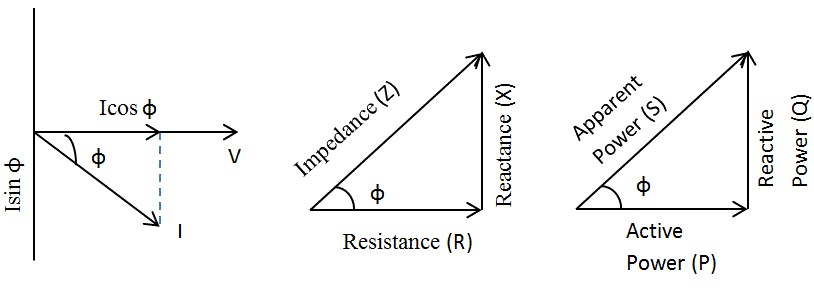
\includegraphics[scale=0.375]{Phasor_Power_Triangle.jpg} % Can't do figure because floats aren't allowed in multicol
		\label{fig:Phasor/Power Triangle}
	\end{multicols}
	\vspace{-4mm}

	\begin{table}[h!] % Complex Power Table
		\centering
		\renewcommand{\arraystretch}{1.4}
		\begin{tabular}{|c|c|c|c|}
			\hline
			\textbf{Name} & \textbf{Symbol} & \textbf{Equation(s)} & \textbf{Units} \\ \hline
			Complex Power & $\mathbf{S}$ & $\frac{P}{Pf} \angle\arccos\left( Pf\right)=P+\jmath Q=\mathbf{V}_{rms} \mathbf{I}_{rms}^{*} = \lvert \mathbf{V}_{rms}\rvert \lvert \mathbf{I}_{rms}\rvert \angle \left( \theta_v - \theta_i\right) $ & VA \\ \hline
			Apparent Power & $S$ & $\lVert \mathbf{S} \rVert = \lvert \mathbf{V}_{rms} \rvert \lvert \mathbf{I}_{rms} \rvert = \sqrt{P^2 + Q^2}$ & VA \\ \hline
			Real Power & $P$ & $\Re\lbrace \mathbf{S} \rbrace = S * Pf = S \cos\left( \theta_v - \theta_i \right)$ & W \\ \hline
			Reactive (Imaginary) Power & $Q$ & $\Im\lbrace \mathbf{S} \rbrace = S \sin \left( \theta_v - \theta_i \right)$ & VAR\\ \hline
			Power Factor &\textit{Pf} & $\frac{P}{S} = \cos(\theta_v - \theta_i)$ & Lead/Lag \\ \hline
		\end{tabular}
	\end{table}
	\vspace{-4mm}

\section*{Elements} \label{sec:Circuit Elements}
	\begin{table}[h!] % Element Equation Table
		\centering
		\renewcommand{\arraystretch}{1.4}
		\begin{tabular}{|c|c|c|c|}
		\hline
		Relation & R & C & L \\
		\hline
		v-i & $V=IR$ & $v = \frac{1}{C} \int_{t_0}^t i(x)dx + v(t_0)$ & $v=L\frac{di}{dt}$  \\
		i-v & $I=\frac{V}{R}$ & $i = C\frac{dv}{dt}$ & $i=\frac{1}{L}\int_{t_0}^t v(x)dx +i(t_0)$ \\
		\hline
		P or W & $P=I^2R=\frac{V^2}{R}$ & $P=\frac{1}{2}Cv_{c}^2$ & $W=\frac{1}{2}Li_{l}^2$ \\
		\hline
		Series & $R_{eq}=R_1+R_2+\ldots+R_n$ & $\frac{1}{C_{eq}}=\frac{1}{C_1}+\frac{1}{C_2}+\ldots+\frac{1}{C_n}$ & $L_{eq}=L_1+L_2+\ldots+L_n$ \\
		Parallel & $\frac{1}{R_{eq}}=\frac{1}{R_1}+\frac{1}{R_2}+\ldots+\frac{1}{R_n}$ & $C_{eq}=C_1+C_2+\ldots+C_n$ & $\frac{1}{L_{eq}}=\frac{1}{L_1}+\frac{1}{L_2}+\ldots+\frac{1}{L_n}$ \\
		\hline
		@ Steady State & Same (Nothing Happens) & Open Circuit & Short Circuit \\
		\hline
		Phasors & $Z_R=R$ & $Z_C = \frac{1}{j \omega C}$ & $Z_L=j \omega L$ \\
		\hline
		\end{tabular}
	\end{table}

\section*{Methods to Solve Equations} \label{sec:Solve Circuits}
	\subsection*{Nodal Analysis} \label{subsec:Nodal Analysis}
		\begin{enumerate}[noitemsep, nolistsep]
			\item \# of Nodes? $\rightarrow n$
			\item Make one node the reference node. Assign $n-1$ nodal voltages
			\item For a \textbf{voltage} source, write a CONSTRAINT EQUATION (Con. Eq.). If there is a voltage source between 2 non-reference nodes, make that a \textbf{SUPERNODE}.
			\item Write KCL at each node. ($n-1$) equations.
			\item Solve Equations.
		\end{enumerate}
	\subsection*{Mesh/Loop Analysis} \label{subsec:Mesh Analysis}
		\begin{enumerate}[noitemsep, nolistsep]
			\item \# of Nodes? $\rightarrow n$ \# of Branches? $\rightarrow b$ \# of meshes/loops? $\rightarrow b-n+1 = l$
			\item Assign $l$ loop currents.
			\item For \textbf{current} sources, write a CONSTRAINT EQUATION (Con. Eq.). If there is a current source between 2 meshes, that's a \textbf{SUPERMESH}.
			\item Write KVL for each mesh.
			\item Solve Equations.
		\end{enumerate}
	\subsection*{Superposition} \label{subsec:Superposition}
		\begin{itemize}[noitemsep, nolistsep]
			\item \# of sources, $n$, determines the number of equations you will have.
			\item Shut off each source, one at a time, solving for the term that you want.
			\begin{itemize}[noitemsep, nolistsep]
				\item Voltage Source = S.C.
				\item Current Source = O.C.
			\end{itemize}
			\item Sum each of the individual terms together. $\sum_{i=1}^{n} x_{i}$ \vspace{1.5mm}
			\item \textbf{\large THIS IS THE ONLY WAY TO SOLVE FOR A CIRCUIT WITH MULTIPLE SOURCES!!}
		\end{itemize}

	\subsection*{Source Transformations} \label{sec:Source Transforms}
		\textbf{ALL} source transformations obey Ohm's Law. $V=IR$.
		This will \textbf{ONLY} work on impedances in series with \textbf{VOLTAGE} sources, or impedances in parallel with \textbf{CURRENT} sources.

\section*{Thevenin and Norton Equivalencies} \label{sec:Thevenin/Norton}
	\begin{itemize}[noitemsep, nolistsep]
		\item ONLY independent sources - Zero all sources, find $\mathbf{Z}_{eq}$.
		\begin{itemize}[noitemsep, nolistsep]
			\item 0-ing Current Sources = O.C., 0-ing Voltage Sources = S.C.
			\item Look at circuit from load's perspective for $\mathbf{Z}_{eq}$
			\item $\mathbf{V}_{Th}=\mathbf{V}_{OC}$, $\mathbf{I}_{N} = \mathbf{I}_{SC}$
		\end{itemize}
		\item BOTH dependent and independent sources
			\begin{itemize}[noitemsep, nolistsep]
				\item Find $\mathbf{V}_{Th}=\mathbf{V}_{OC}$, $\mathbf{I}_{N}=\mathbf{I}_{SC}$
				\item Solve $\mathbf{Z}_{Th}=\frac{\mathbf{V}_{OC}}{\mathbf{I}_{SC}}$
			\end{itemize}
		\item ONLY dependent sources
			\begin{itemize}[noitemsep, nolistsep]
				\item $\mathbf{V}_{Th}=0$, $\mathbf{I}_{N}=0$
				\item $\mathbf{Z}_{Th}=\mathbf{Z}_{N} \rightarrow$ Attach test source @ load.
				\begin{itemize}
					\item If voltage test source, find current. If current test source, find voltage
				\end{itemize}
				\item $\mathbf{Z}_{Th}=\frac{\mathbf{V}_{Test}}{\mathbf{I}_{Test}}$
			\end{itemize}
		\end{itemize}
\section*{Maximum Power Transfer - AC}
			\begin{itemize}[noitemsep, nolistsep]
				\item $\mathbf{Z}_{Load}=\mathbf{Z}_{Th}^*$, $R_{Th}=\Re\lbrace\mathbf{Z_{Th}}\rbrace$, $R_L= \lvert \mathbf{Z}_{Th} \rvert = \sqrt{R_{Th}^2+\left( X_{Th}+X_{L}\right)^2}$
				\item $P_{max}=\frac{\lvert\mathbf{V}_{Th}\rvert^2}{8R_{Th}}$
			\end{itemize}

\section*{3-Phase Circuits} \label{sec:3-Phase}
	\subsection*{$\Delta$-Y Conversion} \label{subsec:Delta-Y Convert}
You want to get everything into Y formation, because the common neutral allows you to do single-phase analysis.

\section*{Mutual Inductance} \label{sec:Mutual Inductance}
	\subsection*{Equivalent Mutual Inductance}
		\begin{table}[h!] % Mutual Inductance Equivalency Table
			\centering
			\renewcommand{\arraystretch}{2.75}
			\begin{tabular}{|c|c|c|}
			\hline
			Series-\textbf{Aiding} Connection & $L=L_{1}+L_{2}+2M$ & 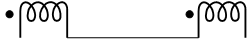
\includegraphics[scale=0.5]{Mutual_Inductors_Series_Dots_Aiding.png} \\ \hline
			Series-\textbf{Opposing} Connection & $L=L_{1}+L_{2}-2M$ & 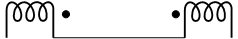
\includegraphics[scale=0.5]{Mutual_Inductors_Series_Dots_Opposing.png} \\ \hline
			\end{tabular}
		\end{table}

	\subsection*{Dot Convention} \label{subsec:Dot Convention}
		There are 2 cases:
		\begin{enumerate}[noitemsep, nolistsep]
			\item Current enters through dotted side on 1 inductor $\longrightarrow$ \textbf{POSITIVE VOLTAGE ON DOTTED SIDE OF OTHER INDUCTOR}
				\begin{itemize}[noitemsep, nolistsep]
					\item Current flows into the dotted side of one inductor
					\item Current flows out of the un-dotted side of second inductor, just like the first
				\end{itemize}
			\item Current enters through \textbf{NON}-dotted side of 1 inductor $\longrightarrow$ \textbf{POSITIVE VOLTAGE ON UN-DOTTED SIDE OF OTHER INDUCTOR}
				\begin{itemize}[noitemsep, nolistsep]
					\item Current flows into the un-dotted side of one inductor
					\item Current flows out of the dotted side of the second inductor, just like the first
				\end{itemize}
		\end{enumerate}
	
	\subsection*{Solving Disjoint Coupled Circuits} \label{subsec:Solve Disjoint Coupled Circuits}
		\begin{enumerate}[noitemsep] % Steps
			\item Apply KVL
			\item Don't forget about the Mutual Inductance Voltage Difference because of the first current
			\item There is a second way to thing about these, shown in Figures~\ref{subfig:Disjoint Coupled Inductors OG}~and~\ref{subfig:Disjoint Coupled Inductors Simplified}, below.
		\end{enumerate}
		\begin{figure}[ht!] % Convert
			\begin{subfigure}{0.5\textwidth}
				\centering
				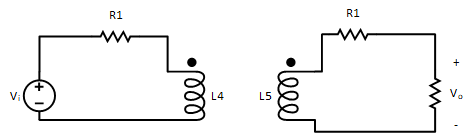
\includegraphics[scale=0.35]{Disjoint_Coupled_Inductors-OG.png}
				\subcaption{Original Circuit}
				\label{subfig:Disjoint Coupled Inductors OG}
			\end{subfigure}
			\begin{subfigure}{0.5\textwidth}
				\centering
				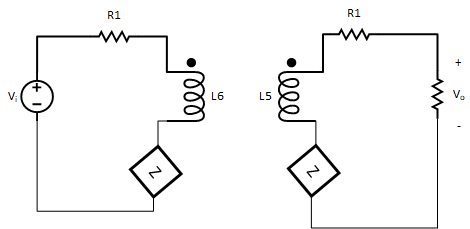
\includegraphics[scale=0.30]{Disjoint_Coupled_Inductors-Simplified.png}
				\subcaption{Circuit "Simplified" by Adding Dependent Sources}
				\label{subfig:Disjoint Coupled Inductors Simplified}
			\end{subfigure}
		\end{figure}
		\textbf{The sign on the dependent sources depends on which side of the inductor the current is going into.} \newline
		\textbf{Use the \nameref{subsec:Dot Convention} to determine which direction the source's voltage should go.}
		
\section*{Transformers} \label{sec:Transformers}
These elements consume no power, and convert voltages and currents.
\begin{itemize}[noitemsep, nolistsep]
	\item $\frac{v_{1}}{v_{2}} = \frac{N_{1}}{N_{2}} \longleftarrow$ Voltage Change
	\item $\frac{i_{1}}{i_{2}} = -\frac{N_{2}}{N_{1}} \longleftarrow$ Current Change
\end{itemize}

	\subsection*{Representations for Turns} \label{subsec:Turn Representations}
		There are 3 common ways to represent the number of turns in a transformer:
		\begin{enumerate}[noitemsep, nolistsep]
			\item $N_{1} : N_{2}$
			\begin{itemize}[noitemsep, nolistsep]
				\item Both $N_{1}$ and $N_{2}$ are integers
			\end{itemize}
			\item $1 : n$
			\begin{itemize}[noitemsep, nolistsep]
				\item The first term might not be $1$, if there isn't perfect division, i.e. $2 : 5$ will not be reduced to $1 : \frac{5}{2}$
				\item $n = \frac{N_{2}}{N_{1}}$
				\item This is the form generally used by our textbook
			\end{itemize}
			\item $a : 1$
			\begin{itemize}[noitemsep, nolistsep]
				\item The second term might not be $1$, if there isn't perfect division, i.e. $2 : 5$ will not be reduced to $\frac{2}{5} : 1$
				\item $a = \frac{N_{1}}{N_{2}}$
				\item This is the form generally used by utility companies
			\end{itemize}
		\end{enumerate}
	
	\subsection*{Reflecting Elements} \label{subsec:Element Reflection}
		There are only 3 equations:
		\begin{enumerate}[noitemsep, nolistsep]
			\item $\frac{v_{1}}{v_{2}} = \frac{N_{1}}{N_{2}} \longleftarrow$ Voltage Change
			\item $\frac{i_{1}}{i_{2}} = -\frac{N_{2}}{N_{1}} \longleftarrow$ Current Change
			\item $Z_{1} = \frac{Z_{2}}{n^{2}}$, as seen in Figure~\ref{fig:Transformer Reflecting}
		\end{enumerate}
		\begin{figure}[ht!]
			\centering
			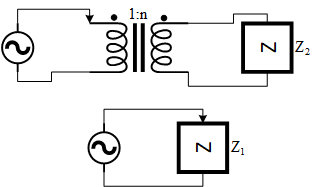
\includegraphics[scale=0.5]{Transformer_Reflecting.png}
			\caption{Transformer Reflecting Elements}
			\label{fig:Transformer Reflecting}
		\end{figure}
	
\section*{Transfer Functions/Bode Plots} \label{sec:Bode Plots}
	\begin{itemize}[noitemsep, nolistsep]
		\item Basic form of a Transfer function is $H \left( \omega \right) = \frac{X_{Out}}{X_{In}}$
		\begin{itemize}[noitemsep, nolistsep]
			\item $H \left( \omega \right) = \frac{V_{Out}}{V_{In}}$
			\item $H \left( \omega \right) = \frac{I_{Out}}{I_{In}}$
			\item $H \left( \omega \right) = \frac{V_{Out}}{I_{In}}$
			\item $H \left( \omega \right) = \frac{I_{Out}}{V_{In}}$
		\end{itemize}
	\end{itemize}
\end{document}